\section{Alternativas de modelamiento\label{sec:alternativas_modelamiento}}

Para cumplir con la definición del problema, se propone un modelo de
programación lineal entera mixta, en el cual se desean obtener la terna de
coordenadas inferior-izquierda-trasera (ver figura~\ref{fig:fig_2_1})
de cada uno de los $i$ objetos en sus componentes $X$, $Y$ y $Z$. \\

\begin{figure}[!htb]
 \centering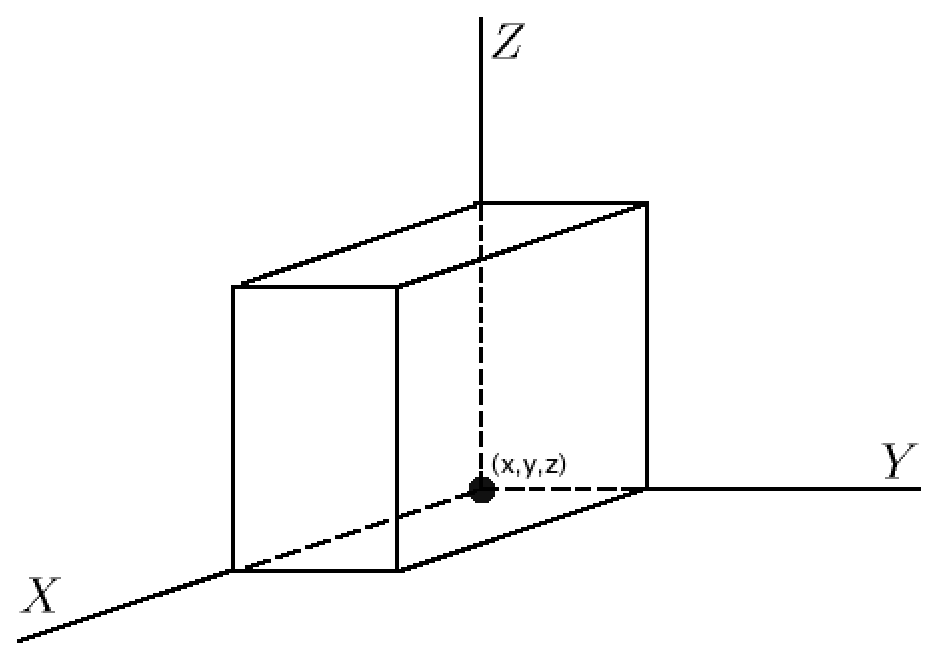
\epsfig{file=fotos/cubo_plano2.eps,width=9cm}
 \caption{Coordenadas $(x,y,z)$ a obtener en la resolución del problema}
 \label{fig:fig_2_1}
\end{figure}

\subsection{Modelamiento}

Un primer acercamiento es considerar la relación que existe entre dos
objetos adyacentes en el espacio, enumerando las posibles combinaciones
de a pares cumpliendo con las restricciones de superposición y contenibilidad
de los objetos dentro de $S_1$. \\

Existen seis restricciones para controlar la superposición de objetos,
estas serán co\-dificadas teniendo en cosideración lo siguiente: \\

\textit{Proposición: Dos objetos $i$ y $j$ no estarán superpuestos si
al menos una de las siguientes restricciones es satisfecha:}
\begin{center}
\begin{tabular}{l p{1cm} c}
Objeto $i$ está a la izquierda de $j$ & & $x_i + w_i \le x_j$ \\
Objeto $i$ está abajo de $j$          & & $y_i + h_i \le y_j$ \\
Objeto $i$ está a la derecha de $j$   & & $x_i - w_j \ge x_j$ \\
Objeto $i$ está arriba de $j$         & & $y_i - h_j \ge y_j$ \\
Objeto $i$ está detrás de $j$         & & $z_i + d_i \le z_j$ \\
Objeto $i$ está delante de $j$        & & $z_i - d_j \ge z_j$ \\
\end{tabular}
\end{center}

Si $H$, $W$ y $D$ son las dimensiones de la superficie $S$, alto, ancho y
profundidad res\-pectivamente, se introducen tres variables binarias
$p_{ij}$, $q_{ij}$ y $r_{ij}$ que permitirán activar solamente una de
las inecuaciones mutamente excluyentes anteriores. \\
\pagebreak

\subsection{Formulación matemática}

Considerando lo anterior, la formulación metamática necesaria para
mantener dos objetos adyacentes sin traslape es la siguiente:

\begin{center}
\begin{tabular}{r c l}
$x_i + w_i$ & $\le$ & $x_j + M \times (p_{ij} + q_{ij} + r_{ij})$ \\
$y_i + h_i$ & $\le$ & $y_j + M \times (1 + p_{ij} + q_{ij} - r_{ij})$ \\
$x_i - w_j$ & $\ge$ & $x_j - M \times (1 + p_{ij} - q_{ij} + r_{ij})$ \\
$y_i - h_j$ & $\ge$ & $y_j - M \times (2 + p_{ij} - q_{ij} - r_{ij})$ \\
$z_i + d_i$ & $\le$ & $z_j + M \times (1 - p_{ij} + q_{ij} + r_{ij})$ \\
$z_i - d_j$ & $\ge$ & $z_j - M \times (2 - p_{ij} + q_{ij} - r_{ij})$ \\
\end{tabular}
\end{center}

Además, es necesario considerar la contenibilidad de los objetos dentro
de la superficie $S_1$, asegurando que no es posible sobrepasar los
límites máximos $H$, $W$ y $D$ de la superficie. \\

\begin{center}
\begin{tabular}{r c l}
$x_i + w_i$ & $\le$ & $W$ \\
$y_i + h_i$ & $\le$ & $H$ \\
$z_i + d_i$ & $\le$ & $D$ \\
\end{tabular}
\end{center}
